\hypertarget{diody_8cpp}{}\section{Dokumentacja pliku diody.\+cpp}
\label{diody_8cpp}\index{diody.\+cpp@{diody.\+cpp}}
{\ttfamily \#include \char`\"{}mainwindow.\+h\char`\"{}}\newline
Wykres zależności załączania dla diody.\+cpp\+:
\nopagebreak
\begin{figure}[H]
\begin{center}
\leavevmode
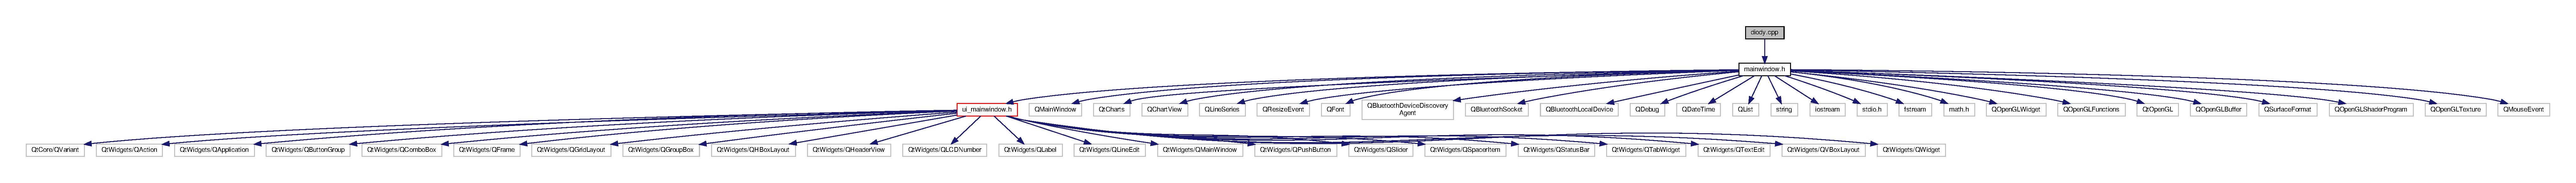
\includegraphics[width=350pt]{diody_8cpp__incl}
\end{center}
\end{figure}
